\documentclass[final]{siamltex}
\usepackage{graphicx}
\usepackage{amsmath}
\usepackage{braket}
\usepackage{latexsym}
\usepackage{bbold,soul}
\usepackage{xcolor}
%\usepackage[T1]{fontenc}
\usepackage[italian]{babel}
\usepackage{amsmath,amssymb}
\usepackage{tikz}
\usepackage{pgfplots}
\usetikzlibrary{shapes,arrows}
\renewcommand{\baselinestretch}{1.0}
\textwidth = 15cm
\usepackage[normalem]{ulem}
\usepackage{cancel}

\begin{document}
\title{Ricostruzione di un'immagine sfocata utilizzando i filtri di Gabor e l'algoritmo \textit{independent component analysis}}
\author{Giacomo Vitali e Marco La Gala}
\maketitle
{\small Progetto didattico per il corso di Analisi Numerica a.a. 2017/2018 - Prof. Simone Fiori\\ 
\\} 
\renewcommand{\thefootnote}{\fnsymbol{footnote}}
\renewcommand{\thefootnote}{\arabic{footnote}}
\def\bbbr{{{\mathbb{R}}}}
\def\bbbs{{{\mathbb{S}}}}
\def\bbbm{{{\mathbb{M}}}}
\def\bbbd{{{\mathbb{D}}}}
\def\bbba{{{\mathbb{A}}}}
\def\bbbc{{{\mathbb{C}}}}
\def\bbbn{{{\mathbb{N}}}}
%
%
\begin{abstract}
Lo scopo di questa relazione \`{e} presentare un metodo che permette di ricostruire un'immagine originale partendo da un'immagine sfocata e di confrontare le differenze tra l'algoritmo \textit{Independent Component Analysis} (ICA) presentato da Shinji Umeyama \cite{Ume} e una sua variante che utilizza le propriet\`{a} dei Manifold su una sfera unitaria. 
\end{abstract}
%
%
%
\begin{keywords}
Ricostruzione di un'immagine sfocata, Filtri di Gabor, Algoritmo Independent Component Analysis, Propriet\`{a} dei Manifold.
\end{keywords}
%
%
%
\section{Introduzione}\label{sec1}
Il processo di ricostruzione di un'immagine consiste nel trovare l'immagine originale partendo da una sua versione sfocata e con disturbi. La sfocatura viene solitamente modellata tramite la convoluzione di un \textit{Point Spread Function} (PSF) con l'immagine originale aggiungendo un ulteriore disturbo. Come \`{e} possibile notare nella Figura \ref{figura1} l'immagine originale \textit{f} dopo essere stata modificata dal PSF diventa un'immagine \textit{g} sfocata.

Se il PSF \`{e} conosciuto a priori si trovano diversi algoritmi che permettono di ricostruire l'immagine mentre, se non \`{e} gi\`{a} noto, la maggior parte degli algoritmi non funziona correttamente in quanto non \`{e} semplice stimare contemporaneamente all'immagine anche il PSF. Esiste un tipo di algoritmo chiamato \textit{Blind Deconvolution} il quale consente di ripristinare l'immagine originale  stimando contemporaneamente sia l'immagine che il PSF. Viene principalmente utilizzato per la ricostruzione delle immagini in astronomia dove si ha la necessit\`{a}, infatti, di migliorare le fotografie ottenute dai telescopi terrestri le quali risultano degradate dalle turbolenze atmosferiche. 
\\
\\
Umeyama, nel suo metodo proposto e discusso in \cite{Ume} e \cite{Umeprecedente}, ha applicato i filtri di Gabor all'immagine sfocata che si deve ricostruire \textit{g}, in modo da scomporla in un numero di immagini filtrate (\textit{Gabor filter 1, \dots , Gabor filter M}). Quest'ultime, insieme all'immagine sfocata $g$, vengono utilizzate in input dall'algoritmo ICA che permette di ottenere un'immagine $f'$ simile all'originale eliminando la sfocatura.
%
\begin{figure}[h!]
\centering
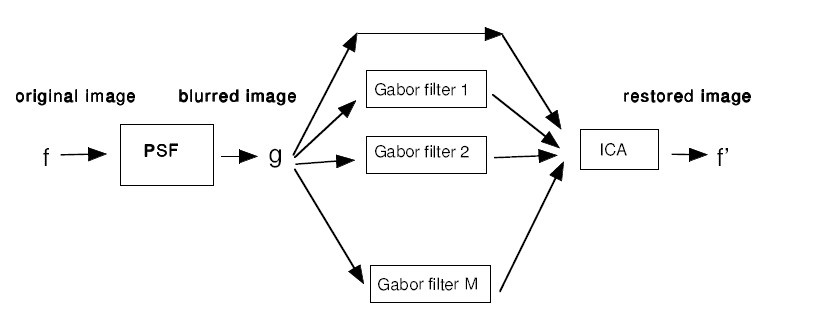
\includegraphics[width=0.9\columnwidth]{Figura1.png}
\caption{Schema dei passi del metodo proposto da Umeyama \cite{Ume}.}
\label{figura1}
\end{figure}
%
\\Negli ultimi anni questo tipo di algoritmo \`{e} stato ampiamente studiato soprattutto nel campo dell'analisi dei dati unidimensionali come per esempio il suono. Nel documento di Umeyama, invece, viene fornita una nuova applicazione per l'analisi dei dati bidimensionali la quale permette di ricostruire un'immagine partendo da una sua versione sfocata senza conoscere il PSF utilizzato. Oltre ad implementare la versione originale dell'algortimo, abbiamo modificato l'algoritmo ICA presente nel documento di Umeyama \cite{Ume} con le nostre conoscenze riguardo i Manifold utilizzando i concetti relativi alla sfera unitaria e alla mappa esponenziale. \\


Di seguito viene fornita una spiegazione dei due metodi utilizzati corredata da esempi con alcune immagini di prova ed un esperimento utilizzando un'immagine realmente sfocata.
%
%
%
\section{Teoria e metodi}\label{sec2} 
%
\subsection{Filtri di Gabor}\label{sec5}
%
I filtri di Gabor, ampiamente utilizzati nel campo della computer vision, realizzano filtri multicanale che possono scomporre un'immagine in un numero di immagini filtrate. I filtri di Gabor di due dimensioni sono costruiti come il prodotto di una funzione Gaussiana 2D e un'onda piana che si propaga su un piano 2D. Ogni filtro \`{e} determinato dalla deviazione standard della funzione gaussiana dalla direzione di propagazione e dalla lunghezza d'onda di un'onda piana. 

I filtri di Gabor in 2D sono definiti come una funzione complessa, dove le parti reali e immaginarie vengono considerate come due filtri reali distinti:

\begin{equation}
\label{eq:gabor1}
R(x,y;\nu,k) = \exp\left(-\frac{x^2+y^2}{2{\sigma_\nu}^2}\right)\cdot \cos\frac{\pi}{\sigma_\nu}\left(x\cos\phi_k+y\sin\phi_k\right),
\end{equation} 
%
\begin{equation}
\label{eq:gabor2}
I(x,y;\nu,k) = \exp\left(-\frac{x^2+y^2}{2{\sigma_\nu}^2}\right)\cdot \sin\frac{\pi}{\sigma_\nu}\left(x\cos\phi_k+y\sin\phi_k\right),
\end{equation} 
%
dove
%
\begin{equation}
\sigma_\nu = \left(\sqrt{2}\right)^{\nu+1} \qquad \mbox{e} \qquad \phi_k = \frac{\pi}{4}k.
\end{equation}
%
Per i nostri esempi abbiamo utilizzato $\nu \in \set{0,1}$ e 
$k \in \set{0,1,2,3}$ come parametri. Otteniamo così 16 filtri di Gabor: 8 reali e 8 immaginari. La Figura \ref{figura2} mostra i filtri che abbiamo implementato stampati come immagini. Le prime due righe mostrano quelli ottenuti imponendo $\nu =0$ mentre le altre due i filtri con $\nu =1$. La prima e la terza riga, inoltre, mostrano i filtri reali $R(x,y;\nu,k)$ che simulano la risposta di un semplice neurone con la capacità di riconoscere una linea mentre la seconda e la quarta quelli immaginari $I(x,y;\nu,k)$ che a loro volta simulano la risposta di un semplice neurone con la capacità di riconoscere un bordo. 

Nelle espressioni \eqref{eq:gabor1} e \eqref{eq:gabor2}, le coppie $(x,y)$ rappresentano le coordinate dei pixel di un'immagine nella forma (colonna, riga).
%
\begin{figure}[h!]
\begin{center}
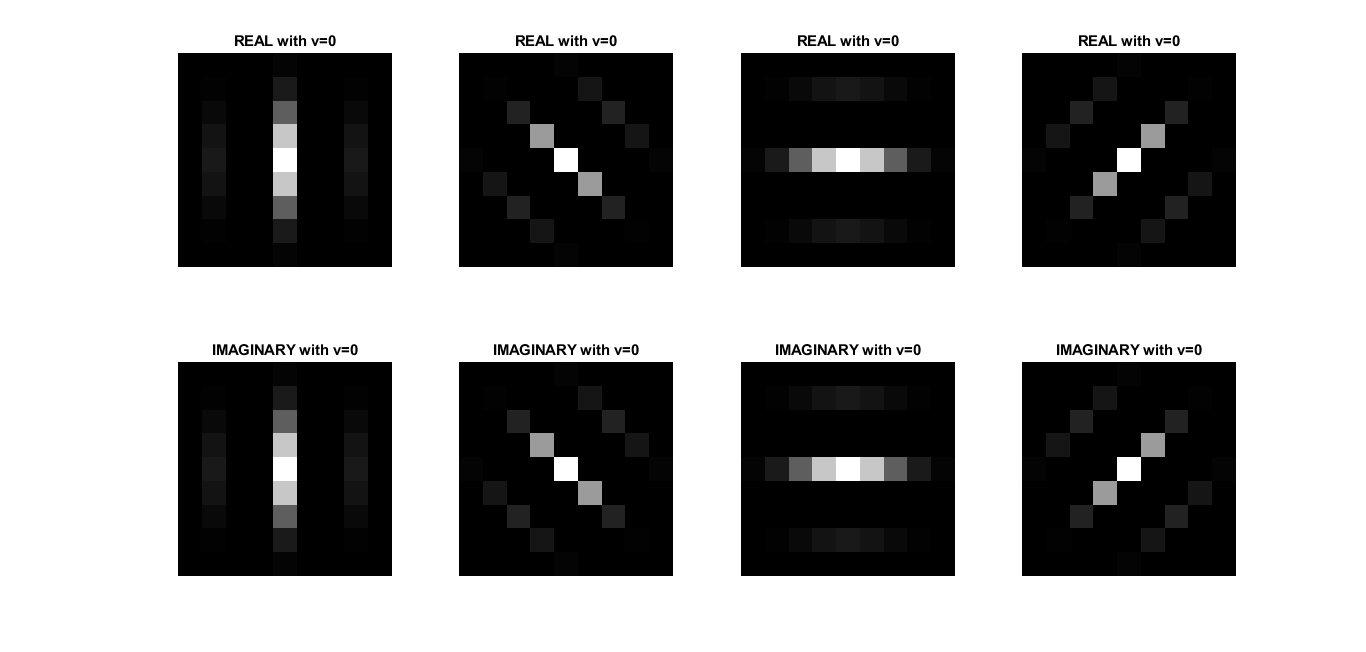
\includegraphics[width=0.9\columnwidth]{Gabor0.png}
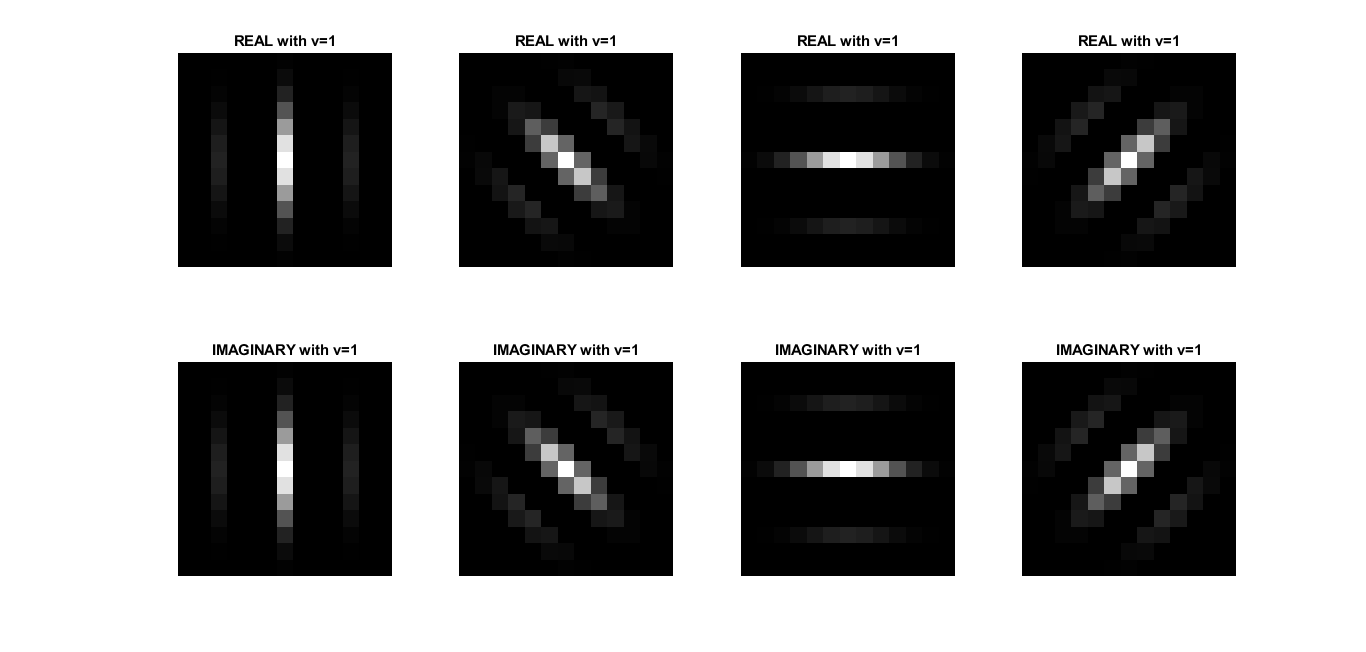
\includegraphics[width=0.9\columnwidth]{Gabor1.png}
\caption{Filtri di Gabor definiti nella Sezione \ref{sec5} con $M=6$.}
\label{figura2}
\end{center}
\end{figure}
%
\begin{figure}[h!]
\begin{center}
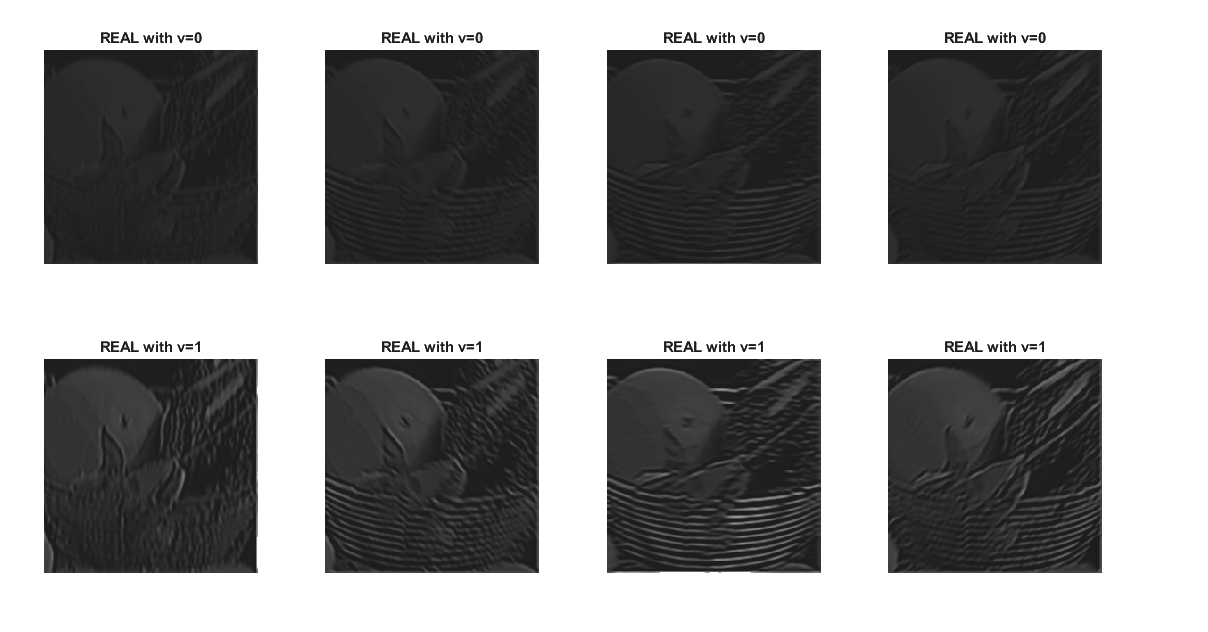
\includegraphics[width=0.9\columnwidth]{gaborfiltrate.png}
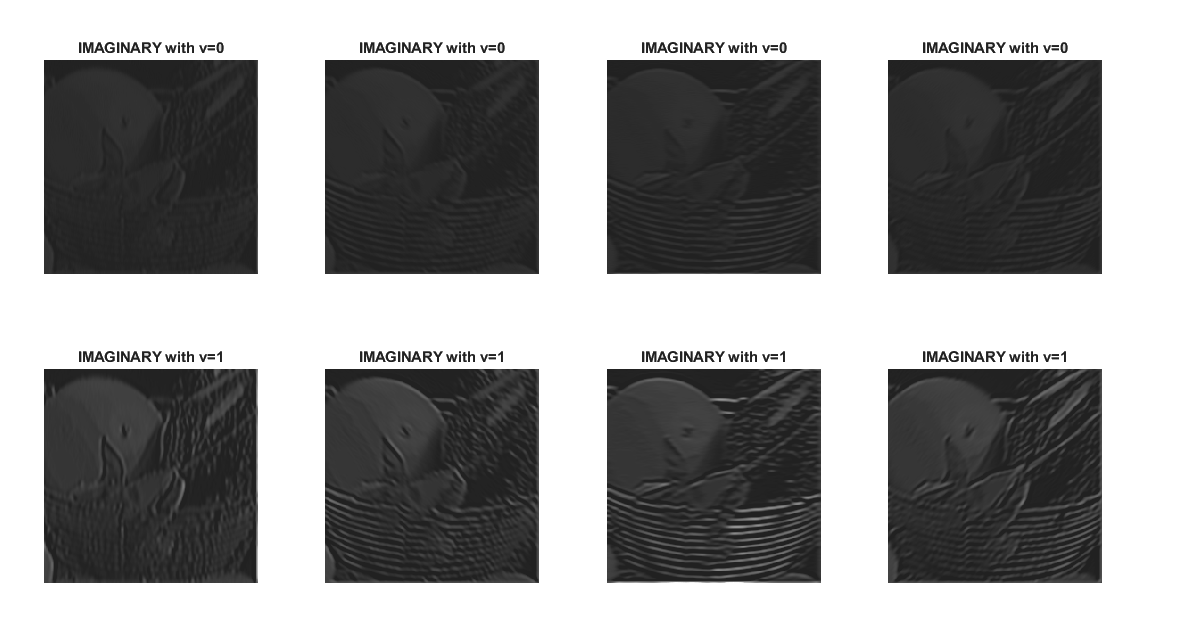
\includegraphics[width=0.9\columnwidth]{gaborfiltrate1.png}
\caption{Immagini ottenute applicando i filtri di Gabor ad un'immagine sfocata.}
\label{gaborfiltrate}
\end{center}
\end{figure}

\newpage
\subsection{\textit{Blind deconvolution} di un'immagine sfocata usando i filtri di Gabor} \label{sec8}
%
Il processo per sfocare un'immagine consiste in una convoluzione tra l'immagine originale $f\left(x,y\right)$ e un PSF $h(x,y)$. Non andremo a considerare il caso in cui l'immagine sfocata da ricostruire abbia, oltre alla sfocatura, un disturbo non prevedibile come per esempio il pulviscolo atmosferico o le polveri sottili presenti nell'aria al momento della foto. 

Si pu\`{o} definire il valore di un pixel $g(x,y)$ dell'immagine sfocata come la somma dei valori dei pixel adiacenti attraverso la convoluzione discreta:
%
\begin{equation}
\label{eq1}
g(x,y) =\sum_{s = -M}^M \sum_{t=-M}^M h(s,t)f(x+s,y+t)
\end{equation}
%
dove $M$ rappresenta l'estensione del PSF ($2M+1$ righe e colonne). Un esempio è mostrato nella Figura \ref{gaborfiltrate}. Allo stesso tempo $f(x+s,y+t)$, che rappresenta il valore di un pixel adiacente, pu\`{o} essere rappresentato come la somma dei valori del pixel centrale $f(x,y)$  e delle sue derivate $f_x(x,y)$ e $f_y(x,y)$ tramite l'espansione di Taylor.
%
\begin{equation}
\label{eq2}
f(x+s,y+t) = f(x,y) + \alpha(sf_x(x,y) + tf_y(x,y) + \dots ).
\end{equation}
%
Usando le equazioni \eqref{eq1} e \eqref{eq2} il valore del pixel $g(x,y)$ pu\`{o} essere approssimato come segue:
%
\begin{equation}
g(x,y) = a_1f(x,y)+a_2f_x(x,y)+a_3f_y(x,y)+ \dots
\end{equation}
%
dove si sono utilizzati i coefficenti 
%
\begin{align}
a_1 & = \quad\sum_{s = -M}^M \sum_{t=-M}^M h(s,t) ,       \\
a_2 & = \alpha\sum_{s = -M}^M \sum_{t=-M}^M s\cdot h(s,t), \\
a_3 & = \alpha\sum_{s = -M}^M \sum_{t=-M}^M t\cdot h(s,t),
\end{align}
$$\dots$$
%
Nel nostro caso specifico abbiamo applicato i filtri di Gabor all'immagine sfocata. Significa che all'immagine originale viene applicata la convoluzione due volte: una con i PSF e l'altra con i filtri di Gabor. Ma questo equivale a fare la convoluzione tra l'immagine originale e una funzione $h' = R*h$ o $h' = I * h$ dove $R$ e $I$ sono i filtri di Gabor rispettivamente reali e immaginari. \\
\\
Quindi possiamo riscrivere, sulle basi delle considerazioni precedenti, l'equazione dell'immagine filtrata con i filtri di Gabor $g'(x,y)$.
%
\begin{equation}
\label{eq3}
g'(x,y) = a_1'f(x,y)+a_2'f_x(x,y)+a_3'f_y(x,y)+ \dots
\end{equation}
%
dove si sono utilizzati i nuovi coefficenti
%
\begin{align}
a_1' &= \quad\sum_{s = -M}^M \sum_{t=-M}^M h'(s,t), \\
a_2' &= \alpha\sum_{s = -M}^M \sum_{t=-M}^M s\cdot h'(s,t), \\
a_3' &= \alpha\sum_{s = -M}^M \sum_{t=-M}^M t\cdot h'(s,t),
\end{align}
$$\dots$$
%
I coefficenti $a_i'$ dipendono dalla forma del filtro di Gabor che abbiamo applicato.
\\
\\
Le equazioni \eqref{eq2} e \eqref{eq3} ci mostrano che l'immagine $g'$ contiene l'immagine originale \textit{f} e le sue derivate $f_x, f_y$. Questo ci porta a pensare che sia possibile ripristinare l'immagine originale (e le sue derivate) quando applichiamo l'ICA alle immagini doppiamente sfocate (sia col PSF che con i filtri di Gabor).
%
%
\subsection{Algoritmo ICA}\label{sec6}
%
Trasformiamo le immagini ottenute (le 16 con i filtri di Gabor e quella sfocata) che non sono altro che matrici $n \times n$, in vettori $g_i$ di dimensione $n^2 \times 1$ tramite una scansione da sinistra a destra e dall'alto verso il basso ottenendo cos\`{i} 17 vettori $g_i^T$, con $i=1, \dots, 17$, i quali andranno a formare una matrice $X$ di dimensione $17 \times n^2$ della seguente forma: 
%
\begin{equation}
X = \begin{bmatrix}
{g_1}^T \\
{g_2}^T \\
\dots \\
{g_{17}}^T \\
\end{bmatrix}
\end{equation}
%
Da notare che le righe che compongono la matrice $X$ sono le 16 immagini ottenute dai filtri e l'immagine sfocata, mentre il numero delle colonne $n^2$ rappresenta il numero totale di pixel di ogni immagine.

Prima di applicare l'algoritmo ICA alla matrice delle immagini $X$ \`{e} utile modificarla attraverso due operazioni chiamate \textit{centering} e \textit{whitening} in modo tale da ottenere migliori prestazioni dell'algoritmo. 

 L'operazione di \emph{centering} consiste nel rendere le colonne della matrice $X$ a valor medio nullo. Scomponiamo, quindi, la matrice $X$ nelle sue $n^2$ colonne, ovvero:
%
\begin{equation}
X=[x_1\ x_2\ x_3\ x_4\ \cdots\ x_{n^2}],
\end{equation}
%
dove ciascun vettore $x_k$  ha dimensione $17\times 1$.
Il valore medio delle $n^2$ colonne della matrice $X$ si calcola come:
%
\begin{equation}
m:=\frac{1}{n^2}\sum_{k=1}^{n^2}x_k,
\end{equation}
%
e le colonne centrate si definiscono come 
%
\begin{equation}
\check{x}_k:=x_k-m.
\end{equation}
%
Indichiamo con $\check{X}$ la matrice le cui colonne sono date dai vettori $\check{x}_k$.


L'operazione di \emph{whitening} consiste nel trasformare linearmente ciascuna colonna della matrice $\check{X}$ in modo da ottenere una nuova matrice $Z=[z_1\ z_2\ z_3\ \cdots z_{n^2}]$ le cui colonne abbiano covarianza unitaria. Si noti che la matrice $Z$ ha dimensione $17\times n^2$. La matrice di covarianza associata alle colonne della matrice $Z$ si definisce come 
%
\begin{equation}
C_z:=\frac{1}{n^2}\sum_{k=1}^{n^2}z_kz_k^T.
\end{equation}
%
Si noti che la matrice $C_z$ ha dimensione $17\times 17$.
Si pu\`{o} verificare che la stessa matrice di covarianza si pu\`{o} calcolare come
%
\begin{equation}
\frac{1}{n^2}ZZ^T=\frac{1}{n^2}(z_1z_1^T+z_2z_2^T+\cdots+z_{n^2}z_{n^2}^T).
\end{equation}


Uno dei metodi diffusi per il whitening \`{e} quello di usare la decomposizione degli autovalori (EVD) della matrice di covarianza 
$ C_z = EDE^T $, dove $E$ \`{e} la matrice ortogonale degli autovettori di $C_z$ e $D$ \`{e} la matrice diagonale degli autovalori $D = diag(d_1, \dots, d_n)$.
\\
\\
Il whitening allora pu\`{o} essere calcolato con la seguente formula
\begin{equation}
\label{eq:whitening}
Z = D^{-1/2}E^T\check{X}
\end{equation}
dove la matrice $D^{-1/2}$ \`{e} calcolata come $D^{-1/2} = diag\left(d_1^{-1/2}, \dots , d_n^{-1/2}\right)$.
\\

Prima di applicare la Formula \eqref{eq:whitening} abbiamo avuto l'accortezza  di eliminare i possibili autovalori inferiori a 0.0001 della matrice $X$, ottenuta dopo l'operazione di \textit{centering},  applicando un restringimento. In particolare abbiamo eliminato i suoi possibili autovalori negativi dovuti a errori numerici. Otteniamo cos\`{i} una matrice $Z$ di dimensione $l \times n^2$ dove $n^2$ rappresenta il numero di pixel dell'immagine utilizzata ed \textit{l} il numero di autovalori presi con il restringimento.

L'algoritmo \textit{Independent Component Analysis} utilizza in input la matrice $Z$ che contiene le varie immagini ottenute dai filtri di Gabor e l'immagine sfocata con le opportune variazioni dovute al \textit{centering} e al \textit{whitening}. La Formula \eqref{eq:ume}, la quale \`{e} la relazione ingresso-uscita di una rete neurale con pesi $w$,  ci permette di ottenere l'immagine restaurata trovando la prima componente indipendente $P$ e consiste nell'applicare il prodotto tra una matrice $w^T$ (di dimensione $1 \times l$) che contiene i pesi di una rete neurale $w$ e una matrice $Z$ ottenuta precedentemente.
%
\begin{equation}
P = w^TZ \qquad(vettore\;1 \times n^2)
\label{eq:ume}
\end{equation}
%
dove il vettore \textit{w} viene modificato con la seguente regola di aggiornamento:
%
\begin{equation}
\label{eq4}
w \leftarrow w+\mu Z\tanh(P^T) 
\end{equation}
%
per poi essere normalizzato
%
\begin{equation}
\label{eq5}
w \leftarrow \frac{w}{||w||}
\end{equation}
%
La Formula \eqref{eq4} e \eqref{eq5} permettono alla rete neurale di apprendere ad eseguire l'algoritmo ICA e vengono iterate pi\`{u} volte fino al raggiungimento di un apprendimento soddisfacente.
 
Impostare un valore del \textit{learning parameter} $\mu$ corretto \`{e} molto importante in quanto permette la convergenza veloce e stabile nei metodi di ottimizzazione non lineari. Se $w$ \`{e} convergente otteniamo la prima componente indipendente. Non abbiamo bisogno delle altre per il problema della \textit{Blind Deconvolution}.
%
%
\subsection{Manifold}\label{sec7}
%
Il \textit{Manifold}, o \textit{variet\`{a}} in italiano, \`{e} uno spazio topologico che localmente ha le caratteristiche di uno spazio Euclideo ma che globalmente pu\`{o} avere propriet\`{a} geometriche molto differenti da esso, ad esempio la curvatura (la quale non \`{e} una propriet\`{a} degli spazi Euclidei).

Un esempio di Manifold unidimensionale potrebbe essere il concetto di linea o cerchio, mentre quello pi\`{u} comune di 2-Manifold (ossia di due dimensioni) \`{e} la sfera. Infatti la terra, vista (localmente) dai suoi abitanti, potrebbe sembrare un piano, ma dallo spazio (globalmente) acquista la forma di una sfera con propriet\`{a} molto diverse da quelle di un piano.  

La propriet\`{a} pi\`{u} significativa dei Manifold  \`{e} che sono una densa collezione di dati astratti ai quali possiamo assegnare delle coordinate \cite{slidefiori}. Questa propriet\`{a} \`{e} mostrata in Figura \ref{imag:manifold1}.\\

Nella nostra applicazione abbiamo utilizzato un tipo particolare di Manifold chiamato \textit{Ipersfera} (\textit{real hyper-sphere}) \cite{documentofiori}, il quale \`{e} definito in maniera seguente:
%
\begin{equation}
S^{n-1} = \{ x \in \mathbb{R}^n \, | \, x^Tx=1 \}
\end{equation}
%
Grazie alle conoscenze riguardo i Manifold, abbiamo pensato a un metodo alternativo per l'aggiornamento del vettore dei pesi $w$ in particolare riguardo la Formula \eqref{eq4} e \eqref{eq5} la quale permette di aggiornare il vettore $w$ per poi normalizzarlo. Visto che il compito dell'algoritmo ICA pu\`{o} essere schematizzato come la ricerca del massimo di una data funzione, lo scopo dell'algoritmo \`{e} cercare il punto di massimo di una funzione su un 2-Manifold, dove il vettore dei pesi $w$ attuale viene aggiornato seguendo il gradiente che rappresenta la direzione di massimo incremento della funzione $f(w)$. \\
%
\begin{figure}[h!]
\begin{center}
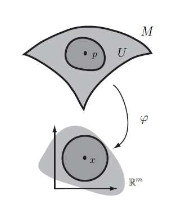
\includegraphics[width=0.3\columnwidth]{manifold1.png}
\caption{Coordinate dei Manifold.}
\label{imag:manifold1}
\end{center}
\end{figure}
% 
%
\begin{figure}[h!]
\begin{center}
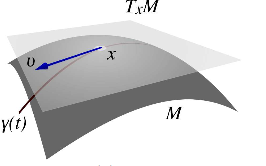
\includegraphics[width=0.3\columnwidth]{manifold3.png}
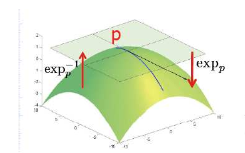
\includegraphics[width=0.3\columnwidth]{manifold4.png}
\caption{Vettore tangente ad un Manifold e mappa esponenziale/mappa logaritmica.}
\label{imag:manifold3}
\end{center}
\end{figure}
%
\\Per questo motivo abbiamo utilizzato il concetto di mappa esponenziale:
%
\begin{equation} 
\label{eq:manifold1}
\exp_x(v)=x\cdot \cos ||v||+ \frac{v\cdot \sin ||v||}{||v||} 
\end{equation}
%
dove $x \in M$ e il vettore tangente $v \in T_xM$. Applicando la mappa esponenziale si ottiene un nuovo punto $q= \exp_x(v)$ (Figura \ref{imag:manifold3}). \\
\\
Utilizziamo anche il concetto di gradiente Riemanniano:
%
{\begin{equation}
\label{eq:manifold2}
\nabla_w f = \left(I - ww^T \right) \frac{\partial f}{\partial w},
\end{equation}
%
dove $\frac{\partial f}{\partial w}$ rappresenta la matrice Jacobiana della funzione $f(w)$ da ottimizzare.\\

Possiamo quindi adattare le Formule \eqref{eq:manifold1} e \eqref{eq:manifold2} secondo lo scopo della nostra applicazione, ottenendo i seguenti risultati:
%
\begin{equation} 
\label{eq:manifold3}
w \leftarrow \exp_w(\mu \nabla_wf )
\end{equation}
%
\begin{equation} 
\label{eq:manifold4}
\exp_w(\mu \nabla_wf )=w\cdot \cos ||\mu \nabla_wf ||+ \frac{\mu \nabla_wf \cdot \sin ||\mu \nabla_wf ||}{||\mu \nabla_wf ||}
\end{equation}
%
\begin{equation} 
\label{eq:manifold5}
\nabla_wf = \frac{1}{n^2} \left(I - ww^T \right) Z \cdot \tanh \left(P^T\right) = \frac{1}{n^2} \left(Z - wP \right) \tanh ^T (P)
\end{equation}
%
Si noti che $ww^T$ \`{e} una matrice $l \times l$, $Z$  \`{e} una matrice $l \times n^2$ e $P^T$ \`{e} un vettore $n^2 \times 1$, mentre il gradiente $\nabla_wf$ \`{e} un vettore $l \times 1$, pertanto le dimensione dell'espressione \eqref{eq:manifold5} sono consistenti. Inoltre la Formula \eqref{eq:manifold3} di aggiornamento del vettore dei pesi \textit{w} ci consente di aggiornare il vettore sulla base di quello attuale e secondo la direzione data dalla formula \eqref{eq:manifold5} del gradiente $\nabla_wf $.\\
La formula \eqref{eq:manifold5} pu\`{o} essere ricavata dalla formula del gradiente Euclideo della funzione $f$ \cite{ICA}:
%
\begin{equation}
f(w) := \mathcal{E}_z[R(w^T z)] = \int R(w^T z) \rho_z(z)dz^{l},
\end{equation}
%
dove $R$ rappresenta una funzione non lineare stabilita da Hyv\"{a}rinen e $\rho_z(z)$ la distribuzione di probabilit\`{a} dei vettori $z$ cio\`{e} degli ingressi della rete neurale ICA (dopo il centering e il whitening). Inoltre, si \`{e} utilizzato l'operatore di ``valore atteso'' (\emph{expectation}) $\mathcal{E}_z[\cdot]$.
Possiamo approssimare l'integrale come una sommatoria con $k$ che da 1 arriva a $n^2$ dove $n^2$ \`{e} il numero di pixel dell'immagine:
%
\begin{equation}
f(w)\approx\sum_{k=1}^{n^2} R(w^T x_k) \mathrm{Pr}(z_k) \Delta z^{l},
\end{equation}
%
dove la quantit\`{a} $\mathrm{Pr}(z_k)$ rappresenta la probabilit\`{a} di incontrare il campione $z_k$ e l'espressione $\Delta z^{l}$ rappresenta il volume di un ``iper-cubetto'' centrato intorno al punto $z_k$.
Calcolando il gradiente Euclideo della funzione $f(w)$ rispetto al vettore $w$, si ottiene:
%
\begin{equation}
\frac{\partial f }{\partial w} = \sum_{k=1}^{n^2} r(w^T z_k)z_k \mathrm{Pr}(z_k) \Delta z^{l},
\end{equation}
%
dove la funzione $r:=R'$ nella nostra applicazione \`{e} data da $r:=\tanh$. Abbiamo quindi ricavato l'equazione \eqref{eq:manifold5}.
Si pu\`{o} vedere anche che, a meno di una costante additiva arbitraria, l'integrale di $r$ risulta $R = \ln \circ \cosh$. 
Per semplicit\`{a}, si pu\`{o} ipotizzare che i campioni $z_k$ siano distribuiti uniformemente, dunque che $\mathrm{Pr}(z_k)=\frac{1}{n^2}$, ottenendo:
%
\begin{equation}
\frac{\partial f }{\partial w} = \frac{\Delta z^{l}}{n^2}\sum_{k=1}^{n^2} \tanh(w^T z_k)z_k.
\end{equation}
%
Infine, conviene osservare che se si lascia che la funzione $\tanh$ agisca componente per componente su un vettore (\emph{component-wise}), risulta:
%
\begin{eqnarray*}
&\frac{1}{n^2}\sum_{k=1}^{n^2}\tanh(w^T z_k)z_k=\\
&\frac{1}{n^2}\left(\tanh(w^T z_1)z_1+\tanh(w^T z_2)z_2+\tanh(w^T z_3)z_3+\cdots+\tanh(w^T z_{n^2})z_{n^2}\right)=\\
&\frac{1}{n^2}Z\tanh(Z^Tw)=\frac{1}{n^2}Z\tanh(P^T)
\end{eqnarray*}
%
e, dunque:
%
\begin{equation}
\frac{\partial f }{\partial w} = \frac{\Delta z^{l}}{n^2}Z\tanh(P^T).
\end{equation}
%
Dato che la quantit\`{a} $\Delta z^{l}$ risulta costante, pu\`{o} essere assorbita nel learning rate $\mu$ ed \`{e} stata, pertanto, ignorata in \eqref{eq:manifold5}.
\\
\\
\\
\section{Risultati degli esperimenti}\label{sec3}
%
\subsection{Risultati degli esperimenti con l'immagine di prova} \label{sec10}
Abbiamo dato in input al nostro programma un'immagine di prova di dimensione $240 \times 240$ mostrata in Figura \ref{imag:gaussian11.png} (a1). \\
Abbiamo creato due PSF:
\begin{itemize}
    \item Gaussian(1,1) con $\theta_x = 1$ e $\theta_y = 1$ mostrati in Figura \ref{imag:gaussian11.png} (a3)
    \item Gaussian(2,2) con $\theta_x = 2$ e $\theta_y = 2$ mostrati in Figura \ref{imag:gaussian22.png} (b3) \\
\end{itemize}
%
%\begin{figure}[h!]
%\begin{center}
%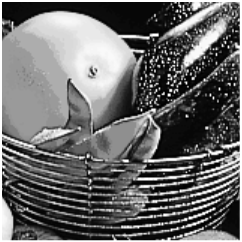
\includegraphics[width=0.22\columnwidth]{originale.png}
%\caption{Immagine originale.}
%\label{imag:originale}
%\end{center}
%\end{figure}
%

Applicando il PSF all'immagine originale, otteniamo l'immagine sfocata mostrata in Figura \ref{imag:gaussian11.png} (a2) per quella creata con il PSF Gaussian (1,1) e in Figura \ref{imag:gaussian22.png} (b2) per quella con il PSF Gaussian (2,2).
Applichiamo ora all'immagine sfocata i filtri di Gabor precedentemente mostrati in Figura \ref{figura2} ottenendo cos\`{i} 16 immagini, le quali insieme all'immagine sfocata, vengono poste in input all'algoritmo ICA.\\
%
\begin{figure}[h!]
\begin{center}
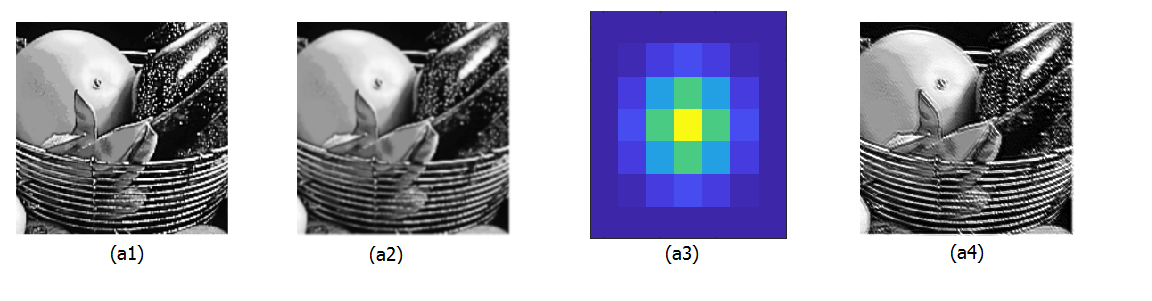
\includegraphics[width=1.1\columnwidth]{totale11.png}
\caption{Immagine originale (a1), sfocata (a2), PSF Gaussian(1,1) (a3), immagine ricostruita (a4). I risultati mostrati sono stati ricavati con l'algoritmo di apprendimento con i Manifold.}
\label{imag:gaussian11.png}
\end{center}
\end{figure}
%
\begin{figure}[h!]
\begin{center}
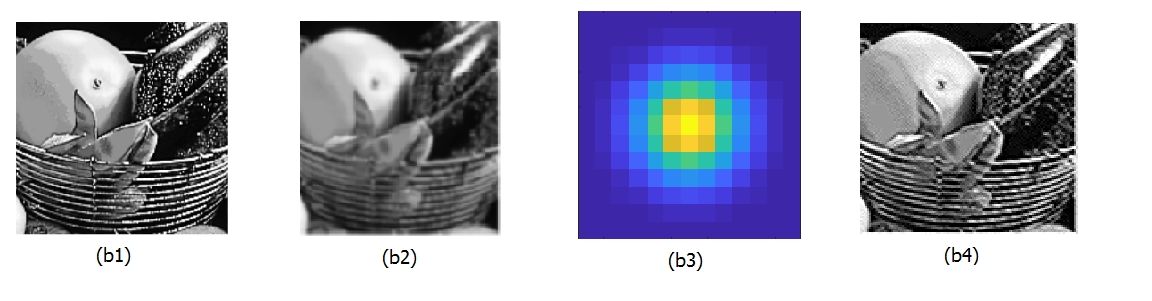
\includegraphics[width=1.1\columnwidth]{totale22.png}
\caption{Immagine originale (b1), sfocata (b2), PSF Gaussian(2,2) (b3), immagine ricostruita (b4). I risultati mostrati sono stati ricavati con l'algoritmo di apprendimento con i Manifold.}
\label{imag:gaussian22.png}
\end{center}
\end{figure}
%
\\
L'algoritmo ICA ci ha restituito un vettore riga $P$ di dimensione $1 \times n^2$ dove $n^2$ \`{e} il numero totale dei pixel di ciascuna immagine. Abbiamo convertito il vettore riga in una matrice $n \times n$ e abbiamo stampato la matrice come immagine. \`{E} possibile vedere il risultato delle due ricostruzioni in Figura \ref{imag:gaussian11.png} (a4) e in Figura \ref{imag:gaussian22.png} (b4). In questo esperimento dopo aver effettuato il centering e il whitening con il relativo restringimento, abbiamo ottenuto una matrice $Z$ di 9 righe ($l=9$). \\

Per il funzionamento corretto dell'algoritmo ICA con i Manifold abbiamo avuto la necessit\`{a} di impostare un \textit{learning parameter} pi\`{u} piccolo affinch\`{e} si possa ottenere un risultato accettabile ($10^{-6}$) rispetto al metodo proposto da Umeyama il quale riesce a far convergere la rete neurale anche con un valore di $10^{-5}$. Per i confronti tra i due metodi abbiamo deciso quindi di imporre il \textit{learning parameter} come 0.00001.\\
\\
Per mostrare la validit\`{a} del metodo abbiamo calcolato i coefficienti di correlazione tra l'immagine originale e l'immagine sfocata, tra l'immagine originale e l'immagine ricostruita dall'ICA di Umeyama e infine tra l'immagine originale e l'immagine ricostruita dall'ICA con i Manifold mostrati nella Tabella  \ref{tab:valori_correlazioneesempi}. 
Notiamo che con i due metodi proposti otteniamo un buon risultato di ricostruzione dell'immagine. Si passa infatti da un valore $0.8836$ a un valore $0.9509$.\\
%
\begin{table}
    \begin{tabular}{| c | c | c | c |} 
    \hline
    PSF utilizzato & Originale/Sfocata & Originale/Restaurata (Umeyama) & Originale/Restaurata (Manifold)  \\
    \hline
   Gaussian(1,1) & 0.9658 & 0.9682 & 0.9684 \\
   \hline
   Gaussian(2,2) & 0.8836 & 0.9484 & 0.9509  \\
   \hline
  \end{tabular}
\label{tab:valori_correlazioneesempi}
\caption{Esempio dei valori di correlazione ottenuti con un'esecuzione del programma.} 
\end{table}
%
\\
Dalla Tabella \ref{tab:valori_correlazioneesempi} si nota subito che il PSF che modifica maggiormente l'immagine è il Gaussian(2,2) e che l'algoritmo che utilizza i concetti dei Manifold riesce a ricostruire meglio l'immagine rispetto all'algoritmo utilizzato da Umeyama. Inoltre, nel caso del PSF Gaussian(1,1), i coefficienti di correlazione tra i due metodi sono pressoch\`{e} identici in quanto il PSF ha dimensioni molto ridotte rispetto all'immagine originale e quindi la sfocature risulta pi\`{u} lieve.\\
%
\begin{figure}[h!]
\begin{center}
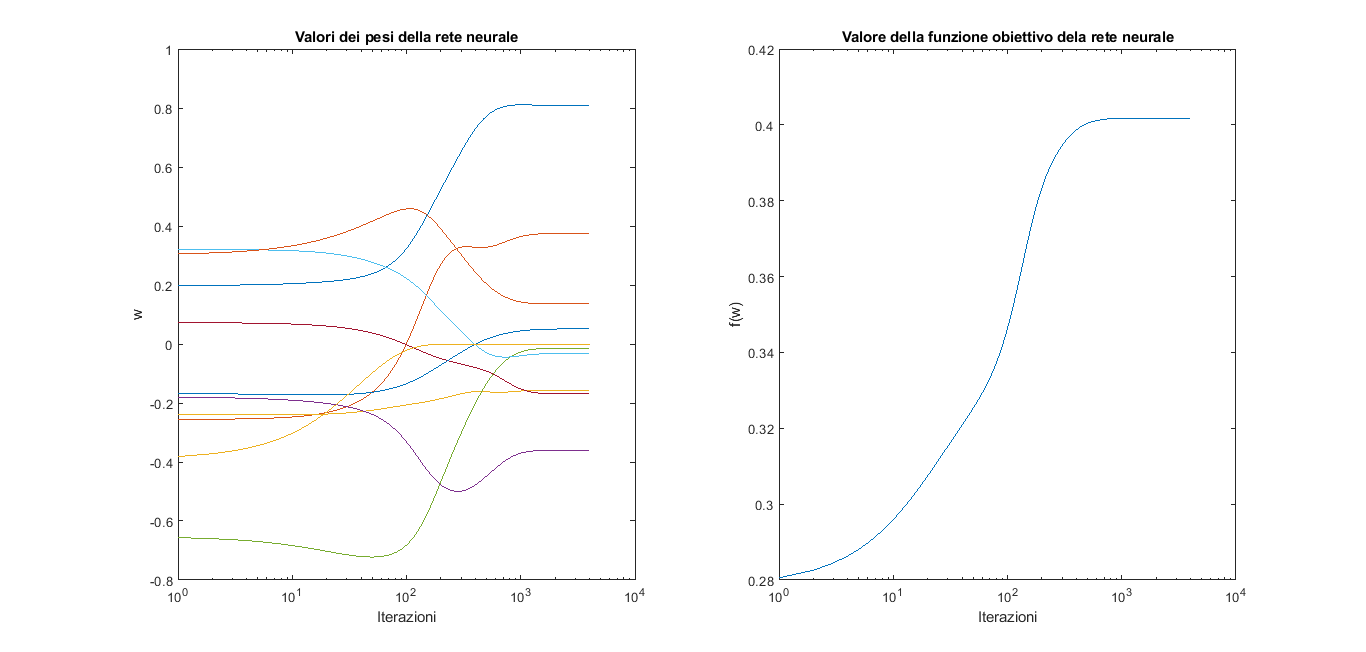
\includegraphics[width=1\columnwidth]{convergenza_reteneurale1.png}
\caption{Grafici di convergenza della rete neurale riferiti all'algoritmo con i Manifold.}
\label{imag:convergenzareteneurale}
\end{center}
\end{figure}
%
\\La Figura \ref{imag:convergenzareteneurale} mostra nel primo grafico la convergenza degli \textit{l} pesi (9 in questo caso) del vettore $w$. Notiamo che il numero di iterazioni \`{e} sufficiente per completare l'operazione in quanto le varie curve convergono intorno a 1000 iterazioni a fronte delle 4000 predisposte. A lato \`{e} inoltre presente il grafico della convergenza della funzione obiettivo $f(w)$ durante l'apprendimento della rete neurale ricavata nel Paragrafo \ref{sec7} ed \`{e} ben visibile la sua convergenza. Possiamo quindi dedurre che il numero di operazioni per l'apprendimento della rete neurale \`{e} sufficiente.\\

Abbiamo, inoltre, calcolato i valori di correlazione medi eseguendo 100 volte il programma che esegue la ricostruzione con i due metodi. Abbiamo generato cos\`{i} 100 vettori dei pesi $w$ i quali sono stati utilizzati dai due metodi, in modo da poter avere una media dei valori di correlazione da poter confrontare. I valori di correlazione medi sono mostrati nella Tabella \ref{tab:valori_medi}.
%
\begin{table}[!htb]
    \begin{tabular}{| c | c | c | c |} 
    \hline
    PSF utilizzato & Originale/Sfocata & Originale/Restaurata (Umeyama) & Originale/Restaurata (Manifold)  \\
    \hline
   Gaussian(1,1) & 0.9658 & 0.9628 & 0.9630 \\
   \hline
   Gaussian(2,2) & 0.8836 & 0.7698 & 0.7728  \\
   \hline
  \end{tabular}
\caption{Valori di correlazione medi calcolati con i PSF utilizzati.}    \label{tab:valori_medi}
\end{table}
%
\\
Come \`{e} possibile notare, il valore di correlazione medio tra l'immagine originale e l'immagine restaurata $0.7698$ \`{e} di gran lunga inferiore a quello tra l'immagine originale e sfocata $0.8836$. Questo significa che i due metodi, nel caso medio, non riescono a migliorare l'immagine sfocata andandola addirittura a peggiorare. 
Questo problema \`{e} dovuto principalmente alla scelta del vettore dei pesi $w$, il quale viene generato casualmente nella prima iterazione per poi essere modificato durante l'apprendimento della rete neurale. In alcuni casi pu\`{o} capitare che il vettore dei pesi $w$ iniziale, essendo casuale, capiti in un'area dove la funzione da massimizzare \`{e} piatta (il gradiente \`{e} quasi zero) e si arresta oppure il numero di iterazioni predisposte dall'algoritmo (4000 nel nostro caso) non sono sufficienti per ricostruire l'immagine. \\

\`{E} possibile vedere un esempio di risultato non ottimale del nostro algoritmo nella Figura \ref{eqnonottimale}: si \`{e} passati da un valore di $0.8836$ ad un valore di $0.7746$ .
%
\begin{figure}[h!]
\begin{center}
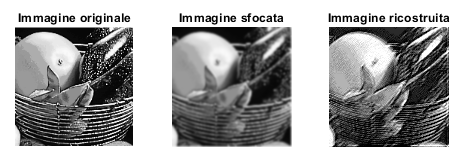
\includegraphics[width=0.7\columnwidth]{eqnonottimale.png}
\caption{Esempio di ricostruzione non completata correttamente.}
\label{eqnonottimale}
\end{center}
\end{figure}
%
\\Per concludere, abbiamo calcolato la convergenza media della rete neurale di entrambi gli algoritmi (eseguendoli 100 volte), in modo da confrontare la velocit\`{a} della loro convergenza. Dalla Figura \ref{reteneurale} possiamo notare come la rete neurale con l'algoritmo di apprendimento con i Manifold converge prima dell'algoritmo proposto da Umeyama. Questo ci porta a dedurre che la convergenza con il primo metodo risulta pi\`{u} veloce del secondo.
%
\begin{figure}[h!]
\begin{center}
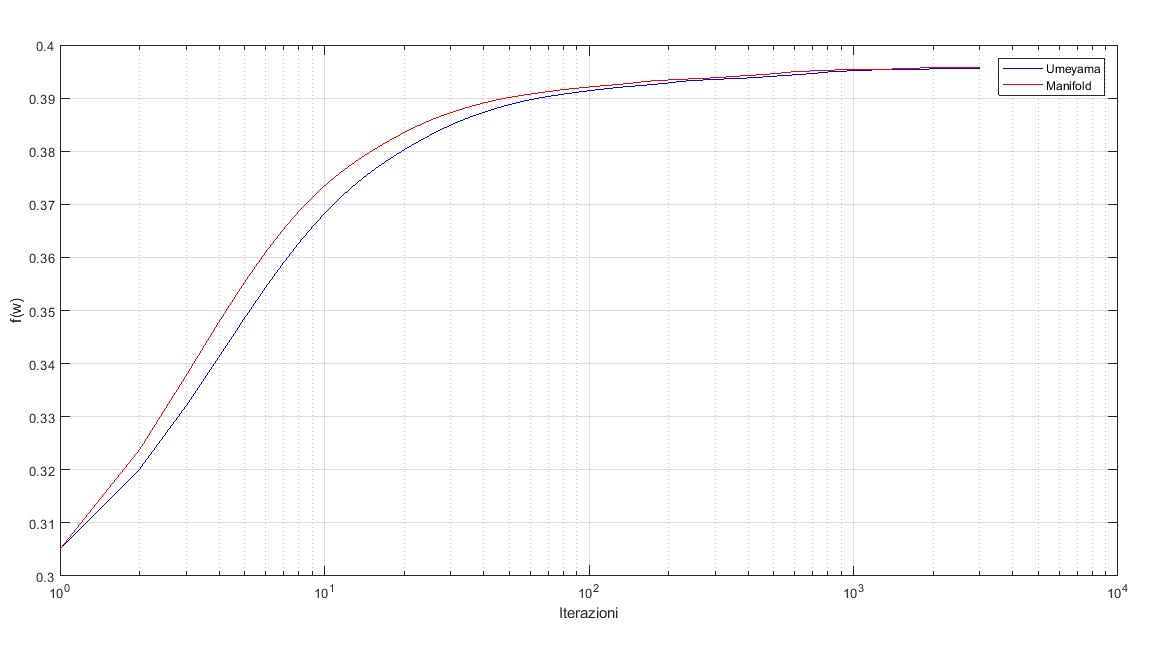
\includegraphics[width=1\columnwidth]{convergenza_reteneurale.png}
\caption{Grafico della convergenza della rete neurale nei due algoritmi studiati, mediato su 100 test indipendenti.}
\label{reteneurale}
\end{center}
\end{figure}
%
\newpage
\subsection{Casistiche in cui il metodo non funziona} \label{sec11}
Il metodo proposto, inoltre, non \`{e} efficiente per tutte le varie tipologie di immagini in quanto se si va ad utilizzarne alcune che  contengono oggetti posti a diverse distanze, come per esempio un paesaggio, il metodo non riesce a ricostruire perfettamente l'immagine andandola addirittura in alcuni casi a peggiorare come è possibile vedere in Figura \ref{imag:nonfunziona}.

\begin{figure}[h!]
\begin{center}
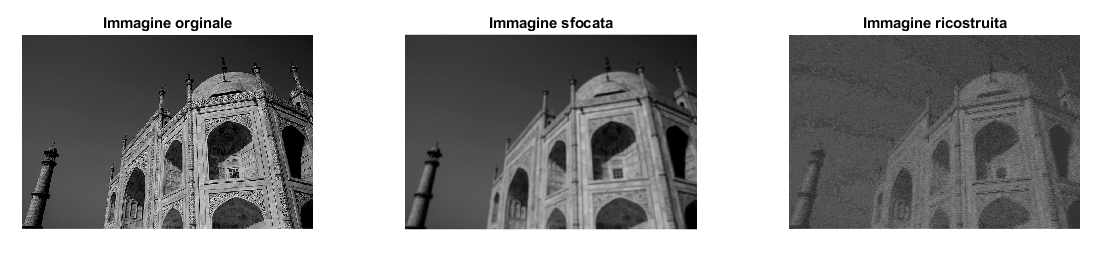
\includegraphics[width=1\columnwidth]{monumento.png}
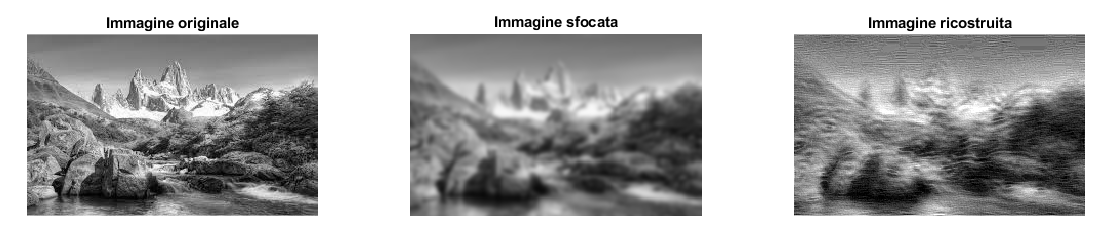
\includegraphics[width=1\columnwidth]{paesaggio.png}
\caption{Le immagini di un monumento e di un paesaggio non vengono correttamente ricostruite dal metodo.}
\label{imag:nonfunziona}
\end{center}
\end{figure}
%
%
%
\subsection{Ripristino di un'immagine realmente sfocata} \label{sec12}
Per un'ulteriore verifica della correttezza del procedimento abbiamo applicato i due metodi a un'immagine realmente sfocata (senza quindi utilizzare il PSF). 
Di seguito \`{e} mostrata una foto di alcuni libri scattata con una macchina fotografica senza essere messa a fuoco. Abbiamo processato l'immagine con i 16 filtri di Gabor e l'output dei filtri, insieme all'immagine originale, viene dato in input all'ICA. L'immagine restaurata con i due metodi \`{e} mostrata nella Figura \ref{imgsfocata}. Come si può vedere, i nomi dei libri che prima non erano distinguibili sono ora leggibili come ad esempio il nome dell'autore del libro centrale \textit{Dan Brown}.  \`{E} importante sottolineare che per utilizzare questo metodo serve che il PSF sia uniforme su tutta l'immagine e per questo motivo abbiamo fotografato dei libri con la stessa profondit\`{a}, in modo da non incorrere nei problemi enunciati nella Sezione \ref{sec11}. Si \`{e} dimostrato quindi che i due metodi possono essere ulteriormente studiati ed approfonditi per future applicazione reali.

\begin{figure}[h!]
\begin{center}
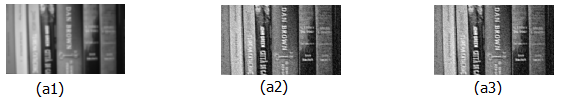
\includegraphics[width=1\columnwidth]{immagine_reale.png}
\caption{Immagine realmente sfocata ricostruita dai metodi studiati. L'immagine mostra rispettivamente la foto sfocata (a1), la foto ricostruita dall'algoritmo di Umeyama (a2) e la foto ricostruita dall'algoritmo con i Manifold (a3).}
\label{imgsfocata}
\end{center}
\end{figure}

Per completezza, nella Figura \ref{imag:3.3nonbella} mostriamo che il risultato della ricostruzione di un'immagine reale ripresa non frontalmente non \`{e} soddisfacente.

\begin{figure}[h!]
\begin{center}
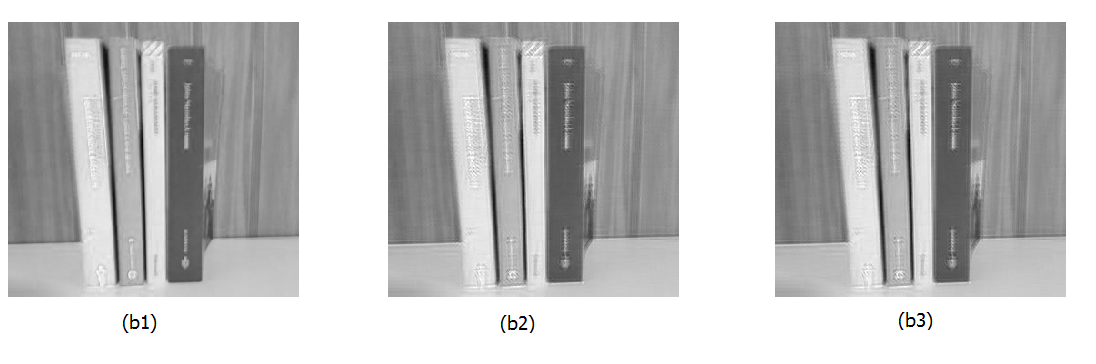
\includegraphics[width=1\columnwidth]{imag3nonbella.png}
\caption{Immagine realmente sfocata ricostruita dai metodi studiati. L'immagine mostra rispettivamente la foto sfocata (b1), la foto ricostruita dall'algoritmo di Umeyama (b2) e la foto ricostruita dall'algoritmo con i Manifold (b3).}
\label{imag:3.3nonbella}
\end{center}
\end{figure}
%
\section{Conclusioni}\label{sec4}
%
In questa relazione abbiamo illustrato il procedimento per la ricostruzione delle immagini proposto da Umeyama e abbiamo fornito una variante con i Manifold utilizzando le conoscenze dell'analisi numerica applicate alle reti neurali e all'\textit{image processing}, in particolare alcune nozioni riguardanti la mappa esponenziale e la sfera unitaria. I due metodi proposti possono ricostruire l'immagine senza conoscere il PSF presente nel modello di sfocatura.

Abbiamo dimostrato nel documento che i metodi riescono a funzionare correttamente ottenendo sotto determinate ipotesi anche un livello di correlazione alto tra l'immagine originale e l'immagine ricostruita, soffermandoci anche sulle motivazioni per cui non si riesce ad ottenere i risultati sperati. Abbiamo dimostrato come la convergenza dell'algoritmo ICA con i Manifold sia pi\`{u} veloce di quella proposta da Umeyama ma allo stesso tempo necessita di una precisione maggiore.

Abbiamo infine fornito un esempio di un'applicazione reale dell'algoritmo ICA, inserendo in input un'immagine gi\`{a} sfocata, notando che se questa viene ripresa frontalmente otteniamo buoni risultati, mentre negli altri casi il risultato non è soddisfacente.

%
\begin{thebibliography}{99}
%

\bibitem{Ume} \textrm{Shinji Umeyama}, Blind Deconvolution of Images using Gabor Filters and Independent Component Analysis, ICA2003, Nara, Japan.
\bibitem{Umeprecedente} \textrm{Shinji Umeyama}, Blind deconvolution of Blurred Images by Use of ICA, Electronics and Communications in Japan, Part 3, Vol.84, No. 12,2001.
\bibitem{ICA} \textrm{Aapo Hyvärinen and Erkki Oja}, Independent Component Analysis: A Tutorial, April 1999.
\bibitem{documentofiori} \textrm{Simone Fiori}, On vector averaging over the unit hypersphere, 17 July 2008.
\bibitem{slidefiori} \textrm{Simone Fiori}, Introduction to Curved Spaces (Manifolds), Lecture 1: Smooth manifolds, curves and tangent spaces.

%
\end{thebibliography}
%
%
\end{document} 
